%%%%%%%%%%%%%%%%%%%%%%%%%%%%%%%%%%%%%%%%%
% Template
% LaTeX Template
% Version 1.0 (December 8 2014)
%
% This template has been downloaded from:
% http://www.LaTeXTemplates.com
%
% Original author:
% Brandon Fryslie
% With extensive modifications by:
% Vel (vel@latextemplates.com)
%
% License:
% CC BY-NC-SA 3.0 (http://creativecommons.org/licenses/by-nc-sa/3.0/)
%
% Authors:
% Sabbir Ahmed
% 
%%%%%%%%%%%%%%%%%%%%%%%%%%%%%%%%%%%%%%%%%

\documentclass[paper=usletter, fontsize=12pt]{article}
%%%%%%%%%%%%%%%%%%%%%%%%%%%%%%%%%%%%%%%%%
% Contract Structural Definitions File Version 1.0 (December 8 2014)
%
% Created by: Vel (vel@latextemplates.com)
% 
% This file has been downloaded from: http://www.LaTeXTemplates.com
%
% License: CC BY-NC-SA 3.0 (http://creativecommons.org/licenses/by-nc-sa/3.0/)
%
%%%%%%%%%%%%%%%%%%%%%%%%%%%%%%%%%%%%%%%%%

\usepackage{geometry} % Required to modify the page layout
\usepackage{multicol}
\usepackage{amsmath}
\usepackage{amssymb}

\usepackage[pdftex]{graphicx}
\usepackage{wrapfig}
\usepackage[font=scriptsize, labelfont=bf]{caption}
\usepackage[utf8]{inputenc} % Required for including letters with accents
\usepackage[T1]{fontenc} % Use 8-bit encoding that has 256 glyphs

\usepackage{avant} % Use the Avantgarde font for headings
\usepackage{courier}
\usepackage{xparse}
\usepackage{xcolor}
\usepackage{listings}  % for code verbatim and console outputs

\setlength{\textwidth}{16cm} % Width of the text on the page
\setlength{\textheight}{23cm} % Height of the text on the page
\setlength{\oddsidemargin}{0cm} % Width of the margin - negative to move text left, positive to move it right
\setlength{\topmargin}{-1.25cm} % Reduce the top margin

\setlength{\parindent}{0mm} % Don't indent paragraphs
\setlength{\parskip}{2.5mm} % Whitespace between paragraphs
\renewcommand{\baselinestretch}{1.5}

\definecolor{green}{rgb}{0.18, 0.55, 0.34}

\graphicspath{ {figures/} }
\captionsetup[table]{skip=10pt}

\lstset{language=C, keywordstyle={\bfseries \color{black}}}

% defines algorithm counter for chapter-level
\newcounter{nalg}[section]

%defines appearance of the algorithm counter
\renewcommand{\thenalg}{\thesection .\arabic{nalg}}

% defines a new caption label as Algorithm x.y
\DeclareCaptionLabelFormat{algocaption}{Algorithm \thenalg}

% defines the algorithm listing environment
\lstnewenvironment{pseudocode}[1][] {
    \refstepcounter{nalg}  % increments algorithm number
    \captionsetup{font=normalsize, labelformat=algocaption, labelsep=colon}
    \lstset{
        breaklines=true,
        mathescape=true,
        numbers=left,
        numberstyle=\scriptsize,
        basicstyle=\footnotesize\ttfamily,
        keywordstyle=\color{black}\bfseries,
        keywords={input, output, return, parallel, function, for, to, in, if,
        else, foreach, while, and, or, new, print},
        xleftmargin=.04\textwidth,
        #1
    }
}{}

\renewcommand{\familydefault}{\sfdefault}  % default font for entire document
 % specifies the document layout and style

\begin{document}

    \documentinfo{\textbf{Question:} 11}{\textbf{DATE:} \today}{Sabbir Ahmed}
    \vspace{-0.1in}

    \section{Background}
    Implement as a strictly combinatorial module ALU that will add or subtract two 5-bit two-signed values a and b based on a control signal sub. The outputs should be a 5-bit two’s-complement result y and an over-/under-flow bit c. Implement two variations of this module using
    \begin{enumerate}[label=\alph*)]
        \item structurally using full 1-bit adders that are in turn built from Verilog primitives
        \item using behavioral code with arithmetic operators
    \end{enumerate}

    \section{Implementation}
        \subsection{Structurally Using Full 1-bit Adders That Are In Turn Built From Verilog Primitives}
        The structural version of the 5-bit adder/subtractor was built using basic gates. Circuit diagrams were used as a reference to minimize the number of gates and ensure accurate outputs. A full 1-bit adder was implemented as a separate module and imported into the circuit design.

        The module implementation along with its test bench can be found in the `scripts' directory. A sample of the waveform generated is provided:

        \begin{figure}[ht]
            \begin{center}
                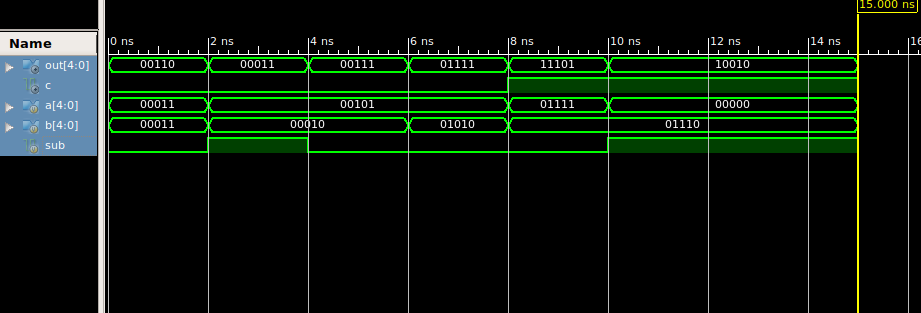
\includegraphics[width=1\textwidth]{struct_wav.png}
                \caption{Waveform Generated from Part 11 Structural Version Test Bench} \label{fig:struct_wav}
            \end{center}
        \end{figure}

        \begin{table}[h]
            \caption{Inputs and Outputs of The Part 11 Structural Version Test Bench}

            \centering
            \begin{tabular*}{200pt}{@{\extracolsep{\fill}} ccccc}

            \textbf{a} & \textbf{b} & \textbf{sub} & \textbf{c} & \textbf{out} \\
            \hline
            00011 ( 3) & 00011 ( 3) & 0 & 0 & 00110 ( 6) \\
            00101 ( 5) & 00010 ( 2) & 1 & 0 & 00011 ( 3) \\
            00101 ( 5) & 00010 ( 2) & 0 & 0 & 00111 ( 7) \\
            00101 ( 5) & 01010 (10) & 0 & 0 & 01111 (15) \\
            01111 (15) & 01110 (14) & 0 & 1 & 11101 (29) \\
            00000 ( 0) & 01110 (14) & 1 & 1 & 10010 (18) \\
            \end{tabular*}
        \end{table}

        \newpage

        \subsection{Using Behavioral Code With Arithmetic Operators}
        The behavioral version of the 5-bit adder proved to be a much simpler implementation, requiring much fewer lines of code.

        The module implementation along with its test bench can be found in the `scripts' directory. A sample of the waveform generated is provided:

        \begin{figure}[ht]
            \begin{center}
                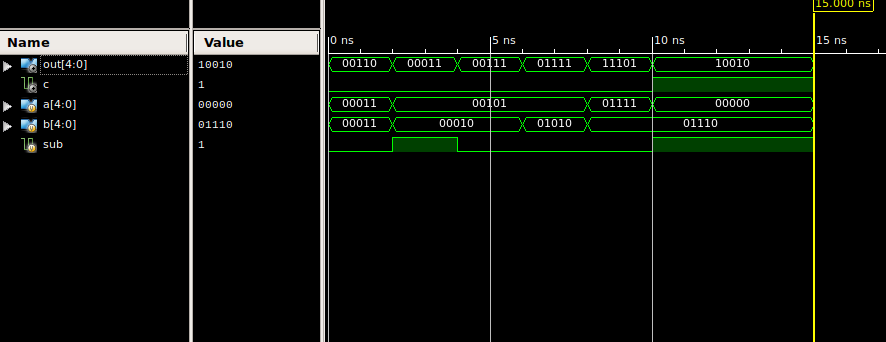
\includegraphics[width=1\textwidth]{behave_wav.png}
                \caption{Waveform Generated from Part 11 Behavioral Version Test Bench} \label{fig:behave_wav}
            \end{center}
        \end{figure}

        \begin{table}[h]
            \caption{Inputs and Outputs of The Part 11 Behavioral Version Test Bench}

            \centering
            \begin{tabular*}{200pt}{@{\extracolsep{\fill}} ccccc}

            \textbf{a} & \textbf{b} & \textbf{sub} & \textbf{c} & \textbf{out} \\
            \hline
            00011 ( 3) & 00011 ( 3) & 0 & 0 & 00110 ( 6) \\
            00101 ( 5) & 00010 ( 2) & 1 & 0 & 00011 ( 3) \\
            00101 ( 5) & 00010 ( 2) & 0 & 0 & 00111 ( 7) \\
            00101 ( 5) & 01010 (10) & 0 & 0 & 01111 (15) \\
            01111 (15) & 01110 (14) & 0 & 1 & 11101 (29) \\
            00000 ( 0) & 01110 (14) & 1 & 1 & 10010 (18) \\
            \end{tabular*}
        \end{table}

    \section{Observations}
    Both the versions of the implementation provided identical outputs. The structural implementation proved to be the more difficult of the 2 versions because of its requirement of understanding the physical design of multi-bit adders and subtractors. A basic comparison in the behavioral version of the implementation appeared to be equivalent to using several gates in the structural version.

\end{document}
